\documentclass[dvipdfmx]{jsarticle}
\usepackage{amsmath,amsfonts}
\usepackage{titlesec}
\usepackage{graphicx}
\usepackage{float}
\usepackage{comment}
\usepackage{fancyhdr}
\usepackage{url}

\lhead{}%ヘッダ左上を空白化
\graphicspath{{../fig/}}%\includegraphicsのファイル名省略用
%高さの設定
\setlength{\textheight}{\paperheight}%ひとまず紙面を本文領域に
\setlength{\topmargin}{-5.4truemm}%上の余白を20mm(=1inch-5.4mm)に
\addtolength{\topmargin}{-\headheight}%
\addtolength{\topmargin}{-\headsep}%ヘッダの分だけ本文領域を移動させる
\addtolength{\textheight}{-40truemm}%下の余白も20mmに
%%幅の設定
\setlength{\textwidth}{\paperwidth}%ひとまず紙面を本文領域に
\setlength{\oddsidemargin}{-0.4truemm}%左の余白を20mm(=1inch-5.4mm)に
\setlength{\evensidemargin}{-0.4truemm}%
\addtolength{\textwidth}{-50truemm}%右の余白も20mmに

%図,表の表示名
\renewcommand{\figurename}{Fig. }
\renewcommand{\tablename}{Table }

%図,表,式などの間隔
\setlength{\abovecaptionskip}{1mm}	%図・表とキャプションの間隔の変更
\setlength{\belowcaptionskip}{1mm}
\setlength{\abovedisplayskip}{3pt}%式の上部のマージン
\setlength{\belowdisplayskip}{3pt}%式の下部のマージン

%図番号を(subsection).(図番号)に変更
\makeatletter
\renewcommand{\thefigure}{\thesection.\arabic{figure}}
\@addtoreset{figure}{section}

%表番号を(subsection).(表番号)に変更
\renewcommand{\thetable}{\thesection.\arabic{table}}
\@addtoreset{table}{section}

%式番号を(subsection).(式番号)に変更
\renewcommand{\theequation}{\thesection.\arabic{equation}}
\@addtoreset{equation}{section}
\makeatother

%注釈
\renewcommand\thefootnote{*\arabic{footnote}}

%目次の表示レベル設定
\setcounter{tocdepth}{3}


\renewcommand{\postpartname}{章} %部を章に変更
%\renewcommand{\thepart}{\Roman{part}}  

\begin{document}

\twocolumn[
  \begin{center}
    \vspace{20mm}
    {\huge 研究計画書}\\
    \vspace{5mm}  
    {\Large 車輪に依存しない段差踏破ロボットの開発}\\
    \vspace{5mm}
    {\Large 千葉工業大学 先進工学部 未来ロボティクス学科 米田研究室}\\
    {\Large 学生番号 21C1016 稲葉健}\\
    \vspace{5mm}
    {\Large \today}\\
  \end{center}
]

\section{研究背景}
近年普及の進む掃除ロボットを始めとする室内移動系のロボットは、車輪径・車高を大きくすることが難しいケースも少なくない。
しかし、一般的な車輪ロボットでは、車輪半径の半分以上、車高以上の段差を登攀することは困難である。
そのため、現行の室内移動ロボットの運用は、大きな段差のないフロアを移動することが主である。
% 画像
\begin{figure}[H]
  \centering
  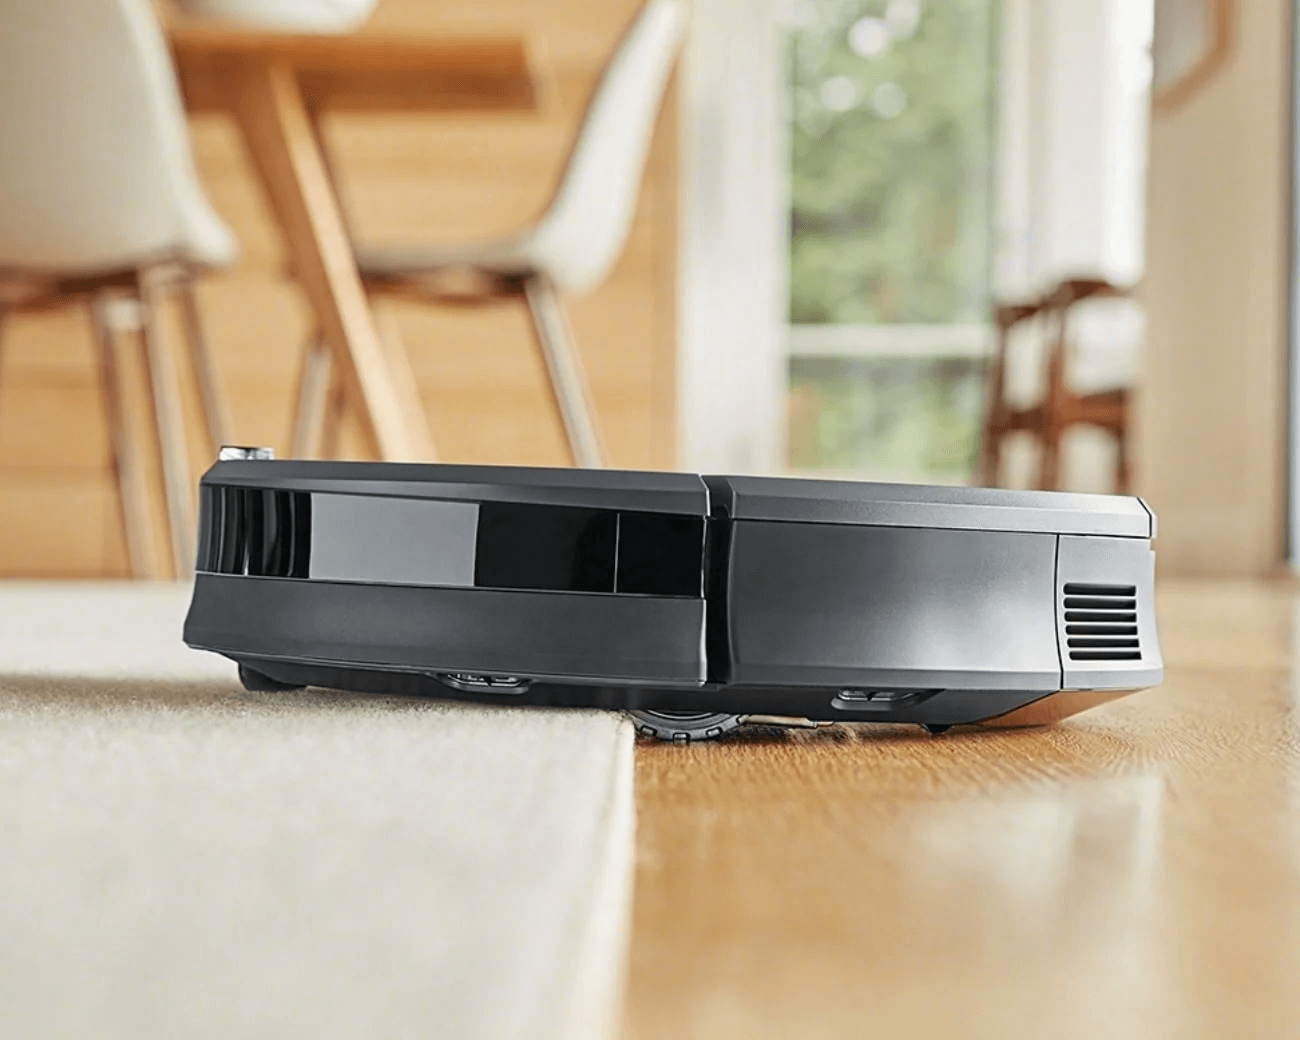
\includegraphics[width=50mm]{image/roomba.png}
  \caption{段差を乗り越えるルンバ}
  \label{fig:runba}
\end{figure}
したがって、室内移動型のロボットを複数階建ての一軒家などで運用する場合、
複数のフロアで稼働させるためには人間がロボットを移動させるか、別フロアの作業は人間が行う必要がある。
移動させる作業はロボットの重量が増えていくごとに困難になり、
作業中の事故なども懸念される。
また、人間が代わりの作業を行うとなると、ロボットを導入したメリットを享受できるのが1フロアだけになってしまう。

そこで、車輪で移動を行い、段差の上り下りを車輪に依存せずに行うロボットを開発すれば、
車輪径や車高は別の問題に最適化しつつ、フロア移動が可能になるのではないかと考えた。
\section{研究目的}
現在普及の進む掃除ロボットの中には段差登攀性能を売りにしている製品も存在する。
しかし、Fig.\ref{fig:rulo}に示すようにその多くが$20\mathrm{mm}$程度のカーペットやラグなどで生じる小さな段差を想定しており、
階段サイズの段差を登攀可能な製品は少ない。
% 画像
\begin{figure}[H]
\centering
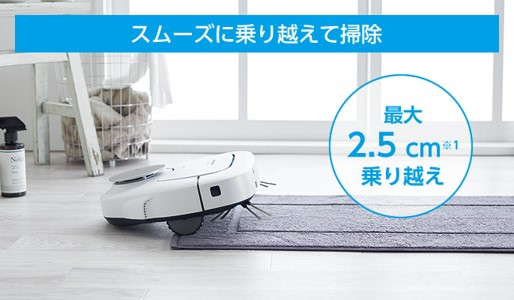
\includegraphics[width=50mm]{image/rulo.jpg}
\caption{東芝 rulo}
\label{fig:rulo}
\end{figure}

一般的な階段の段差は約$200\mathrm{mm}$程度であり、奥行きは$300\mathrm{mm}$程度ある。

本研究では一般家庭の階段を連続登攀することを想定し、直径$300\mathrm{mm}$の円内に全長が収まり、
$200\mathrm{mm}$の段差登攀性能を有すロボットの開発を目的とする。
また、車輪径については、iRobot社のルンバの車輪径よりも小さい$55\mathrm{mm}$径のものを使用し、
既存のロボットにも応用可能であることを示す。

\section{研究方法}
段差踏破方法について、二つのユニットを用いて互いを持ち上げ合う方式を取る。

Fig.\ref{fig:model01}に示すように、二つのユニットをアームし、上の段に登った
ユニットに重りを移動させ、段差の下のユニットを持ち上げることで段差の登攀を完了する。
登攀の際に移動させる重りの条件式である。
% 数式
\begin{equation}
  M=\frac{l'+lcos\theta-l''}{l''}m
\label{equ:model01}
\end{equation}
変数はそれぞれ、 
Mは移動させる重りの質量、
mは機体重量(各ユニットの重量)、
l'は重りの乗っていないユニットの重心からリンク節までの距離、
l''はユニットと重り込みの重心からリンク節までの距離、
lは二つのユニットにまたがるリンク間距離である。
式(\ref*{equ:model01})より、Mを最小限に抑えるには持ち上げる瞬間のlcos$\theta$を小さくする必要があることが分かる。
そのため、アームの中央に自由度を追加し、したユニットの持ち上げ時にはFig.\ref{fig:model02}
の様にアームを畳み込み、モーメントを減少させる。
% 画像
\begin{figure}[H]
  \centering
  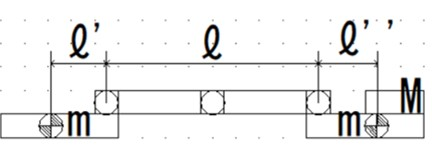
\includegraphics[width=50mm]{image/model01.jpg}
  \caption{機体模式図}
\label{fig:model01}
\end{figure}
\begin{figure}[H]
  \centering
  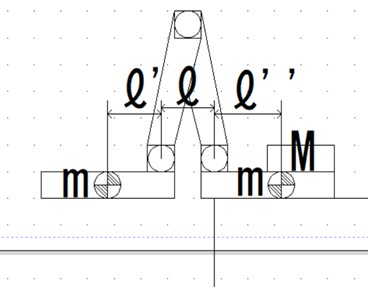
\includegraphics[width=50mm]{image/model02.jpg}
  \caption{登攀動作模式図}
\label{fig:model02}
\end{figure}

重りの移動について、アームが3自由度であり、
各ユニット間の距離が不定になるため、液体をポンプで輸送する方法を採用する。

\section{スケジュール}
\section{期待される効果}
\section{大学院での抱負}


\end{document}
